\documentclass[english,nofirstpagebreak,empty]{amsproc}
\usepackage{amsmath}
\usepackage[cdot,amssymb]{SIunits}
\usepackage{verbatim}
\usepackage{graphicx}
\usepackage{tikz}
\usepackage{pgflibrarysnakes}
%%%%%%%%%%%%%%%%%%%%%%%%%%%%%%%%%%%%%%%%%%%%%%%%%%%%%%%%%%%%%%%%%%%%%%%%%%
%%%%%%%%%%%%%%%%%%%%%%%%%%%%%%%%%%%%%%%%%%%%%%%%%%%%%%%%%%%%%%%%%%%%%%%%%%



%%%%%%%%%%%%%%%%%%%%%%%%%%%%%%%%%%%%%%%%%%%%%%%%%%%%%%%%%%%%%%%%%%%%%%%%%%
%%%%%%%%%%%%%%%%%%%%%%%%%%%%%%%%%%%%%%%%%%%%%%%%%%%%%%%%%%%%%%%%%%%%%%%%%%


\begin{document}

\title[Modeling of a  Rectangular Flow Cell]{Modeling and Simulation
of  Coupled  Species  Transport, Porous  Electrode  Effects  and
Catalytic Reactions in a
Rectangular Flow Cell}

\date{April 15, 2008}

\author{
J\"urgen Fuhrmann \and
Hong Zhao \and
Hartmut Langmach  \and
Ekkehard Holzbecher}

\begin{abstract}
  For the  cross-section through a  two-dimensional thin layer
  flow  cell, we  present  a model  which  allows us to  take into  account
  kinetics of catalytic reactions including the dynamics of the catalyst
  covering,  transport  and  reactions   of  a  dissolved  reagent,  and
  electrochemical effects  in a porous electrode  including double layer
  capacity.   The  model has  been  implemented  using  a finite  volume
  method. Besides  transient calculations, the  calculation of cyclic
  voltammograms and impedance spectra,  which are measurement
  methods  used   by  electrochemists, is possible.
\end{abstract}


\keywords{ Finite  Volumes,
Electrochemistry, Flow Cell}

\maketitle
%%%%%%%%%%%%%%%%%%%%%%%%%%%%%%%%%%%%%%%%%%%%%%%%%%%%%%%%%%%%%%%%%%%%%%%%%%
%%%%%%%%%%%%%%%%%%%%%%%%%%%%%%%%%%%%%%%%%%%%%%%%%%%%%%%%%%%%%%%%%%%%%%%%%%
\section{Introduction}

Thin layer flow cells are electrochemical devices which can be used to
measure electrochemical  reaction kinetics. In order  to conclude from
the  measurement  to   actual  kinetic  parameters,  coupling  between
reactive and transport processes  needs to be regarded. Traditionally,
in such  situations, asymptotic theory based on  boundary layer theory
was  successfully invoked  \cite{Leveque1928,Levich1962}  in order  to
model  such situations.   In  thin  layer flow  cells,  just by  their
geometrical dimensions, the actual thickness of the cell can correlate
with  the  thickness  of   the  boundary  layer,  thus  rendering  the
prerequisites      of     the     asymptotic      approach     invalid
\cite{FuhrmannZhaoEtAl2008xUlm}.                                     In
\cite{FuhrmannZhaoHolzbecherLangmach2008},   we  proposed   a  coupled
transport-reaction model  for such a process and  demonstrated that it
can be used for inverse modeling of reaction parameters.

In this  paper, we  extend this model  in order to  include electrical
conductance in  the electrolyte and  the porous electrode layer  to be
measured.   More   precisely,  we   basically  couple  the   model  of
\cite{FuhrmannZhaoHolzbecherLangmach2008}  with  the porous  electrode
theory \cite{Newman+ThomasAlyea-2004}.  This model extension allows us to
take  into account  the effects  of the  electrochemical  double layer
which forms around  the grains of the porous  electrode. The inclusion
of this effect is important when precise comparisons to time dependent
measuring   approaches   like   cyclic   voltammetry   and   impedance
spectroscopy are intended.

The  numerical method  is  implemented using  a  Voronoi box  centered
finite  volume  method on  boundary  conforming  Delaunay meshes.   It
includes the  options for  numerical simulation of  cyclic voltammetry
and impedance spectroscopy.  In  electrochemistry, as in other fields,
impedance  spectroscopy  is  interpreted  using  equivalent  circuits.
Here, we demonstrate the feasibility  of an approach which is based on
the  numerical model, and  demonstrate its  applicability to  the flow
cell model.


As  an advantage  of  the presented  approach  we see  the ability  to
guarantee  local mass  conservation and  a discrete  maximum principle
\cite{EymardFuhrmannGaertner2006}.   Numerical   methods  for  similar
problems have been developed by  other groups as well.  For example, a
finite difference approach  has been taken in \cite{AldenCompton1997}.
Adaptive  finite elements  resp. discontinuous  Galerkin  methods have
been         used         in         \cite{HarrimanGavaghanSueli2004},
\cite{GavaghanGillowSueli2006}.

%%%%%%%%%%%%%%%%%%%%%%%%%%%%%%%%%%%%%%%%%%%%%%%%%%%%%%%%%%%%%%%%%%%%%%%%%%
%%%%%%%%%%%%%%%%%%%%%%%%%%%%%%%%%%%%%%%%%%%%%%%%%%%%%%%%%%%%%%%%%%%%%%%%%%
\section{The model}
\begin{figure}[b]
  \centering
  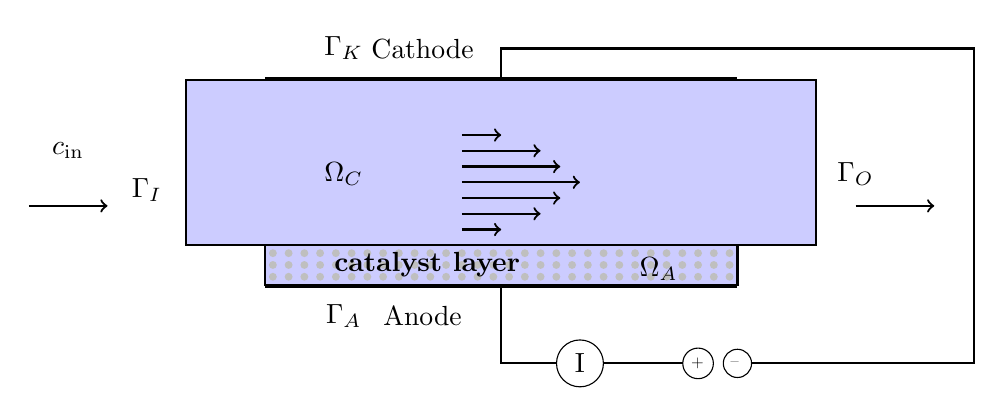
\begin{tikzpicture}
      \begin{scope}[scale=1]
        \draw[->,thick] (-2,1)-- (-1,1);
        \draw[->,thick] (8.5,1)-- (9.5,1);
        
        \draw  (-1.5, 1.7) node{$c_{\text{in}}$};
      
        \draw  (-0.5, 1.2) node{$\Gamma_I$};
        
        \draw (8.5,1.4)    node{$\Gamma_O$};
        
        \draw[thick,fill=blue!20]  (0,0.5) rectangle (8,2.6);
        \draw[thick,fill=blue!20]  (1,0) rectangle (7,0.5);
        
        \path (5,-1) node[circle,draw](I) {I};
        \path (6.5,-1) node[circle,draw,scale=0.5,text width=1em]
                      (plus) {\large +};
        \path (7,-1)   node[circle,draw,scale=0.5,text width=1em]
                      (minus) {\large --};
        

        \draw[thick] (4,2.6)-- (4,3) -- (7,3) -- (10,3) -- (10,-1) --
                   (minus.east);
        \draw[thick] (1,-0.025) -- (7,-0.025);
        \draw[thick] (1,2.625) -- (7,2.625);
        
        
        \draw[thick] (4,0) -- (4,-1) --  (I.west) ;
        \draw[thick] (I.east) -- (plus.west) ;
        \foreach \pos in {1.1,1.3, ..., 6.9} 
        { \fill[fill=gray!50] (\pos,0.1) circle(0.05cm);
          \fill[fill=gray!50]  (\pos,0.25) circle(0.05cm);
          \fill[fill=gray!50]  (\pos,0.4) circle(0.05cm);
        }
        \draw (3,0.25) node{{ \textbf{catalyst layer}}};
        \draw[->,thick]  (3.5,0.7) -- (4,0.7);
        \draw[->,thick]  (3.5,1.9) -- (4,1.9);
        
        \draw[->,thick]  (3.5,0.9) -- (4.5,0.9);
        \draw[->,thick]  (3.5,1.7) -- (4.5,1.7);
        
        \draw[->,thick]  (3.5,1.1) -- (4.75,1.1);
        \draw[->,thick]  (3.5,1.5) -- (4.75,1.5);
        
        \draw[->,thick]  (3.5,1.3) -- (5,1.3);
        
        \draw  (2, 1.4) node{$\Omega_C$};
        \draw  (6, 0.2) node{$\Omega_A$};
        \draw  (3, -0.4) node{Anode};
        \draw  (3, 3) node{Cathode};
        \draw  (2, 3) node{$\Gamma_K$};
        \draw  (2, -0.4) node{$\Gamma_A$};
      \end{scope}
    \end{tikzpicture}
    {\small \textbf{Figure 1.} \emph{Simplified 2D model of a flow cell}}
    \label{fig:flowcell}
  \end{figure}
  

The  domain   under  consideration  (see   Figure  \ref{fig:flowcell})
$\Omega=\Omega_A\cup \Omega_C$ consists consists of the the the anodic
porous catalyst layer $\Omega_A$,  and the flow domain $\Omega_C$. The
boundary                    $\Gamma=\partial                   \Omega=
\Gamma_I\cup\Gamma_O\cup\Gamma_A\cup\Gamma_K\cup\Gamma_N$  consists of
the  inlet  $\Gamma_I$,  the  outlet $\Gamma_O$,  the  anodic  contact
$\Gamma_A$, and the cathodic  contact $\Gamma_K$, and insulating walls
denoted  by $\Gamma_N$.  Constants, unknowns  and units  one  finds in
Table \ref{tab:units}.
\begin{subequations}
We regard the following model:
  \begin{align}
  \partial_t (\varepsilon c) - \nabla\cdot (D\nabla c + c \vec v) 
               & = R_c \quad\text{in}\; \Omega \label{eq:tran}\\
 \partial_t C_{dl}(\phi_h-\phi_e) - \nabla\cdot \sigma_h\nabla\phi_h
                    &=R_\phi\quad\text{in}\; \Omega \label{eq:prot}\\
 \partial_t C_{dl}(\phi_e-\phi_h) - \nabla\cdot \sigma_e\nabla\phi_e
                           &=-R_\phi\quad\text{in}\; \Omega_A
\label{eq:ele}
  \end{align}
\end{subequations}

Equation \eqref{eq:tran} describes  diffusion, transport and reaction
of $H_2$ dissolved in a  dilute electrolytic solution which is flowing
through the flow chamber. The $H_2$ concentration is denoted by $c$ and
is  defined  in  $\Omega_A\cup  \Omega_C$.   As the  flow  chamber  is
rectangular,  we  assume  Hagen-Poiseuille  flow in  $\Omega_C$.   The
simplifying  assumption of zero  flow in  the porous  layer $\Omega_A$
removes   the   need   to   couple   fluid   flow   to   Darcy's   law
\cite{FuhrmannZhaoHolzbecherLangmach2008}.  The  resulting flow vector
field
\begin{equation} 
 \vec v(\vec x)= 
\begin{cases}
     \vec v(\vec x)=(v_1, v_2)=(4v_{max}\frac{x_2}{h}(1-\frac{x_2}{h}),0) & \vec x \in \Omega_C\\
     0 ,&  \vec x \in \Omega\setminus\Omega_C
  \end{cases}
\end{equation} is  continuous and divergence-free in  the whole domain
$\Omega$.   Equation \eqref{eq:prot} describes  Ohm's law  for protons
($H^+$  ions)  in  the  electrolyte  under  the  assumption  of  local
electro-neutrality.  These  are represented by  their potential $\phi_h$
defined  in  $\Omega_A\cup  \Omega_C$.   Equation  \eqref{eq:ele}  is
responsible  for the  charge transport  in  the porous  matrix of  the
catalyst.  The  electrons are represented by  their potential $\phi_e$
defined  in   $\Omega_A$.   Corresponding  to   the  classical  porous
electrode theory  \cite{Newman+ThomasAlyea-2004}, both Ohm's  laws are
coupled in $\Omega_A$  by the Faradaic reaction term  $R_\phi$ and the
double layer charge  $C_{dl}(\phi_h-\phi_e)$ (in $\Omega_C$, we assume
$C_{dl}=0$ and $R_\phi=0$).


In the simplest case, the oxidation of $H_2$ on a $Pt$ catalyst can be
modeled      using      the      Volmer-Tafel      mechanism 
\cite{HamannVielstich1998}
\begin{subequations}
  \begin{align}  
    H_2 +2 S &\rightleftharpoons  2 H_{ad}  &&
         \text{$H_2$ adsorption} \label{eq:had}\\
    H_{ad} & \rightleftharpoons  H^+ +e^- +S 
&&\text{$H_2$ oxidation + desorption}\label{eq:hdes}.
  \end{align}
\end{subequations}  where $S$  represents  a free  catalyst site,  and
$H_{ad}$ denotes the adsorbed hydrogen.

In  order  to  describe  the  kinetic expressions,  we  introduce  the
normalized      occupation     numbers      of      catalyst     sites
$\theta_{H}=\frac{c_{H_{ad}}}{c^{eff}_{Pt}}$ and the normalized number
of  free  catalyst sites  $\theta_{Pt}=  1-\theta_{H}$.  Reaction
system \eqref{eq:had}--\eqref{eq:hdes} is then represented by
\begin{subequations}
\begin{align}
r_1 &= k_1^+ \frac{c_{H_2}}{c_{H_2}^{ref}}\theta_{Pt}^2-k_1^- \theta_{H}^2\\
r_2 &= k_2^+  \theta_{H} e^{\alpha \phi F/RT}-k_2^-  a_{H^+}\theta_{Pt}e^{-(1-\alpha)\phi F/RT}
\end{align}
\end{subequations} 

Accordingly,     $R_c=      c_{Pt}^{eff}r_1$     and     $     R_\phi=
\frac{1}{F}c_{Pt}^{eff}r_2$.        To            PDE       system
\eqref{eq:tran} -- \eqref{eq:ele} we add the rate equation for the
catalyst covering
\begin{align}\label{eq:theta}
  \frac {d \theta_{H}}{d t} = 2r_1-r_2 \quad\text{in}\; \Omega_A
\end{align}

We assume that at the inlet $\Gamma_I$, a fixed concentration $c=c_I$ 
defines a Dirichlet boundary condition. At the outlet $\Gamma_O$ we
assume an outflow boundary condition $\partial_n c=0$. The proton
potential has a fixed value $\phi_h=0$ at cathode $\Gamma_K$, and
the electron potential is set to a (possibly time dependent) value
$\phi_e=\Phi(t)$ at the anode $\Gamma_a$.
\begin{table}[t]
  \centering
  \begin{tabular}{lll}
    $c$ & \mole\per\cubic\meter & $H_2$ concentration\\
    $\phi_h$& \volt & proton potential\\
    $\phi_e$& \volt & electron potential\\
    $\vec v$ & \meter\per\second& flow velocity\\
    $\vec v_\text{max}$& $10^{-2}$\centi\meter\per\second & maximal flow velocity\\
    $D$ & $5\cdot 10^{-9}$ \meter\squared\per\second & $H_2$ diffusion coefficient\\
    $c_I$ & 1 \mole\per\cubic\meter & inlet concentration\\
    $\sigma_h$& 5000 \siemens/\meter & protonic conductivity of electrolyte\\
    $\sigma_e$& 20 \siemens/\meter  & electronic conductivity of catalyst matrix\\
    $C_{dl}$ &$10^8$\farad\per\cubic\meter&  double layer capacity\\
    $\varepsilon$& 0.7 &porosity\\
    $h$ & 50 \micro\meter & height of flow chamber\\
    $c^{eff}_{Pt}$& $10^3$\mole\per\cubic\meter & effective
    catalyst concentration\\
    $c^{ref}_{H_2}$& 1\mole\per\cubic\meter &reference
    concentration of hydrogen\\
    $c_{H_{ad}}$ &\mole\per\cubic\meter& concentration of adsorbed
    $H$\\
    $\theta_H$ && hydrogen occupation number\\
    $\theta_{Pt}$& &occupation  number for free catalyst sites\\
    $R$ & $1.38\cdot 10^{-23}$ \joule\per\kelvin &Boltzmann constant\\
    $F$ & 96485.3415 \coulomb\per\mole &Faraday constant\\
    $T$ & 25\celsius & temperature\\
    $\alpha$& 0.5 & kinetic factor\\
    $a_{H_2}$ &1 & proton activity\\
  \end{tabular}
  \caption{Notations, and values of coefficients}
  \label{tab:units}
\end{table}


%%%%%%%%%%%%%%%%%%%%%%%%%%%%%%%%%%%%%%%%%%%%%%%%%%%%%%%%%%%%%%%%%%%%%%%%%%
%%%%%%%%%%%%%%%%%%%%%%%%%%%%%%%%%%%%%%%%%%%%%%%%%%%%%%%%%%%%%%%%%%%%%%%%%%
\section{Finite volume discretization and solution strategy} 

The  finite volume  discretization  of the  system \eqref{eq:tran}  --
\eqref{eq:ele}, \eqref{eq:theta} is fairly straightforward. We choose a
two-point      flux     ansatz      on     an      admissible     mesh
\cite{EymardGallouetHerbin2000}  together   with  the  implicit  Euler
method.   This   includes  the   coupling  to  the   immobile  species
$\theta_H$. The  convective part in \eqref{eq:tran} is  upwinded by an
exponential fitting scheme. The  varying sets of unknowns are handled
using  a dummy  equation approach  \cite{Fuhrmann2002}.  To  create an
admissible mesh, we use  the Voronoi-Delaunay method which consists of
the definition of  the finite volumes by joining  the circumcenters of
the  triangles adjacent  to a  given  vertex by  straight lines.   The
primal triangular meshes are  either generated from rectangular meshes
by  subdividing each  rectangle into  two  halves, or  by using the  mesh
generator triangle \cite{Shewchuk2007}.  Dirichlet boundary conditions
are  implemented using the  boundary penalty  method, and  the outflow
boundary condition  for $c$  is consistently discretized  according to
\cite{FuhrmannLangmach2001}.  Boundary currents are calculated using a
test    function    approach   similar    to    that   described    in
\cite{GaertnerRichter2005}.  The nonlinear  systems occuring  for each
time step  is solved  by Newton's method  with exact jacobians  of the
discrete  nonlinear  problem.   Linear  systems  are  handled  either
iteratively   or  by   the  direct   sparse  matrix   solver  Pardiso
\cite{PARDISO}.
%%%%%%%%%%%%%%%%%%%%%%%%%%%%%%%%%%%%%%%%%%%%%%%%%%%%%%%%%%%%%%%%%%%%%%%%%%
\section{Modeling of electrochemical measurement approaches}
The primary measurement is that of the
anodic current
$
  I=\int_{\Gamma_A} \sigma_e \nabla \phi_e \cdot n ds 
$
for a given applied voltage $\Phi$. Besides 
stationary states and transient responses to a voltage step,
cyclic voltammetry \cite{HarrimanGavaghanSueli2004} and impedance spectroscopy are of importance.
%%%%%%%%%%%%%%%%%%%%%%%%%%%%%%%%%%%%%%%%%%%%%%%%%%%%%%%%%%%%%%%%%%%%%%%%%%


Impedance  spectroscopy  consists  in  measuring  the  response  to  a
periodic  (sinus-like)  applied  voltage  with varying  frequency  and
measuring  the complex  amplification factor  for each  frequency. The
standard way  to interpret these measurements  is based on  the use of
equivalent  electrical circuits. However, a  comprehensive numerical  model of
the process like that presented here allows us to avoid this step
and  to   obtain  a   model  based  interpretation.    Assuming  small
perturbations,  an efficient  implementation  avoiding long  transient
calculations can be performed in the frequency domain.

For a  given time  interval ${\mathbf T}=[0,T]$,  a {\em  state space}
$\mathcal V$, and a finite dimensional {\em parameter space}, $\mathbf
P$, regard the abstract doubly nonlinear evolution equation
\begin{equation}\label{eq:abstrevol}
 \frac{d S(v(t),\lambda)}{dt} + D(v(t),\lambda)=0.
\end{equation}

The  state of  the system  is {\em  measured} by  some  functional $M:
\mathcal V  \rightarrow \mathbf M$, where  $\mathbf M $  is the finite
dimensional {\em  measurement space}. For example,  $\mathcal V$ may
result   from  the   semi-discretization  of   a  system   of  partial
differential equations by the finite volume method.

Given  a steady state  solution $(v_0,  \lambda_0)$ such  that $D(v_0,
\lambda_0)=0$, measured  by $M_0=M(v_0)$, we  would like to  trace its
response  to  a small,  periodic  perturbation $\lambda(t)=  \lambda_a
\exp(i\omega  t)   $.   Expressing   this  response  as   $M(t)=  M_0+
M_a(\omega) \exp(i\omega t)$, we yield the {\em impedance} $Z(\omega)=
M_a(\omega)^{-1} \lambda_a$.



In order  to calculate the  frequency response, we apply  the standard
ansatz of small-signal  analysis $v(t)=v_0+v_a\exp(i\omega t)$ for the
perturbation  of the  state  variable and  calculate  the first  order
Taylor expansions  of the terms  $S,D,R$.  Putting them  into equation
\eqref{eq:abstrevol} and using the steady state condition yields
\begin{equation}\label{eq:comp}
    i\omega\left( 
      S_v(v_0,\lambda_0)v_a+
      S_\lambda(v_0,\lambda_0)\right)+ 
    D_v(v_0,\lambda_0)v_a+
    D_\lambda(v_0,\lambda_0)=0
\end{equation}
for given $\omega$ with the unknown complex function $v_a$.
Assuming $\dim \mathbf M =\dim \mathbf P=1$,
the impedance  can  then be calculated as 
\begin{equation}\label{eq:imp}
  Z(\omega)= \frac1{M_v(v_0)v_a}
\end{equation}

Covering the case of an  applied periodic voltage, assume the periodic
forcing  $\lambda$   occurs  in  a   Dirichlet  boundary  condition
implemented by the penalty  method using penalty parameter $\epsilon$.
Therefore,        we         write        $D(v,\lambda)=        D_i(v)
+\frac1\epsilon\delta_{\Gamma_A}(v-\lambda)$ ($\delta$ denoting
a discrete delta function which is $1$ on nodes belonging to $\Gamma_A$
and 0 elsewhere).  Then
\begin{equation*}
  \begin{split}
    D_v(v,\lambda)= D_{i,v}(v)+  \frac1\epsilon\delta_{\Gamma_A},\quad
    D_\lambda(v,\lambda)= -\frac1\epsilon\delta_{\Gamma_A},
   \end{split}
\end{equation*}
and we have to solve 
\begin{equation*}
  i\omega S_v v_a + D_{i,v} v_a  +\frac1\epsilon\delta_{\Gamma_A}(v_a-1) =0
\end{equation*} 
 which corresponds  to the  Dirichlet problem  for the
linearized equation  with boundary value 1 on  $\Gamma_A$.

Algorithmically, we proceed as follows:
\begin{itemize}
\item   Given $\lambda_0$, solve the steady state equation $D(v_0,\lambda_0)=0$.
\item Obtain Jacobi matrices $D_v(v_0,\lambda_0)$ and $S_v(v_0,\lambda_0)$. % bprime
\item Prepare solution and right hand side with boundary conditions.
\item for $\omega=\omega_0\dots\omega_1$ do
  \begin{itemize}
  \item Set up matrix $i\omega\left( 
      S_v(v_0,\lambda_0)+S_\lambda(v_0,\lambda_0)\right)+ 
    D_v(v_0,\lambda_0)v_a
    D_\lambda(v_0,\lambda_0)$.
\item Solve complex linear system \eqref{eq:comp}.
\item calculate impedance according to \eqref{eq:imp}.
  \end{itemize}
\end{itemize}



For testing  Newton's method with  full analytical Jacobians  has been
chosen  as  a  solution  strategy  in  the  time-dependent  case,  the
derivatives $D_v, S_v$ are  available in a straightforward manner.  If
the functional  $M$ is linear, e.g.   a boundary flux  calculated by a
test  function, it is  sufficient to  use the  complex version  of the
already existing linear code.  In our implementation based on C++, we
conveniently use templates for  maintaining real and complex versions
at once.


For testing this  strategy, we calculate the impedance  of the current
response  at $L$  to  voltage change  in  $0$ of  the linear  reaction
diffusion system in $(0,L)$
  \begin{equation}\label{eq:imptest}
      Cu_t - (Du_x)_x + Ru=0,\quad
      u(0,t)=\lambda,\quad
      u(L,t)=0
  \end{equation}
  As response functions we take the current  $I_L=Du_x(L,t)$.
  The corresponding time domain equation is
    \begin{equation*}
        Ci\omega v - (Dv_x)_x +Rv =0, \quad
        v(0,t)=1,\quad
        v(L,t)=0.
    \end{equation*}
    Setting $z=\sqrt{i\omega\frac{C}{D}+\frac{R}{D}}$, 
    for the solution, we make the ansatz
    $ v=ae^{zx}+be^{-zx}$
    which fulfills the differential equation.
    Setting $e^+=e^{zL},e^-=e^{-zL}$, from the boundary 
    conditions we get
    $ a+b=1 $ and 
   $ ae^++be^- =0$,
   yielding  $a=\frac{e^-}{e^--e^+},b=\frac{e^+}{e^+-e^-}$.
Therefore, we have
\begin{equation*}
  Dv_x(L)=Dz(ae^+-be^-)=Dz\frac{e^-e^++e^+e^-}{e^--e^+}=\frac{2Dz}{e^--e^+}
\end{equation*}

\begin{figure}[t]
  \centering
  \includegraphics[width=0.5\textwidth]{plot-imp}
  \label{fig:plotimp}

  {\small \textbf{Figure 2.} \emph{Comparison of analytically (dots) and numerically (lines)
    obtained values for the impedance of test problem
    \eqref{eq:imptest}.}}
\end{figure}

An implementation of \eqref{eq:imptest} using the same approach as for
the main problem  has been obtained and tested  against the analytical
results.   Here, we  used $L=1,  C=1, D=1$  and varied  $R$.  A visual
comparison can be found in Figure \ref{fig:plotimp} which uses the
Nyquist plot of  $\mbox{\rm im}Z(\omega)$ vs. $\mbox{\rm re}Z(\omega)$
as a standard way to visualize the impedance.




%%%%%%%%%%%%%%%%%%%%%%%%%%%%%%%%%%%%%%%%%%%%%%%%%%%%%%%%%%%%%%%%%%%%%%%%%%
%%%%%%%%%%%%%%%%%%%%%%%%%%%%%%%%%%%%%%%%%%%%%%%%%%%%%%%%%%%%%%%%%%%%%%%%%%
\section{Numerical results}

In order to demonstrate the feasibility of the computational approach,
we present the  result of the calculation of  cyclic voltammograms and
impedance spectra  for the  presented model for  realistic parameters,
typically     taken    from    \cite{DivisekFuhrmannGaertnerJung2003},
\cite{HamannVielstich1998}, \cite{FuhrmannZhaoHolzbecherLangmach2008},
summarized  in  Table   \ref{tab:units}.   The  calculation  has  been
performed on a triangular mesh consisting of 10122 vertices.  

Work  in progress  together with  different groups  of electrochemists
\cite{FuhrmannZhaoEtAl2008xUlm}  is  devoted   to  the  comparison  to
measurements   in   real  flow   cells,   allowing   for  a   thorough
interpretation of  the computational  results and improvements  of the
model.

\begin{figure}[t]
  \centering
  \label{fig:numres}
  \includegraphics[width=0.45\textwidth]{test-cv}
  \includegraphics[width=0.45\textwidth]{test-ny}

  {\small \textbf{Figure 3.} \emph{Left: cyclic voltammetry  sweeps for three different values
of                                                             $v_{max}=
(10^{-2}, 2\cdot10^{-2}, 4\cdot10^{-2})\centi\meter\per\second$.}

\emph{ Right:
Nyquist  plots  of impedance  spectra  for  three  different values  of
applied voltage for $v_{max}=10^{-2}\centi\meter\per\second$.}}
\end{figure}

%%%%%%%%%%%%%%%%%%%%%%%%%%%%%%%%%%%%%%%%%%%%%%%%%%%%%%%%%%%%%%%%%%%%%%%%%%
%%%%%%%%%%%%%%%%%%%%%%%%%%%%%%%%%%%%%%%%%%%%%%%%%%%%%%%%%%%%%%%%%%%%%%%%%%
\bibliographystyle{unsrt}
\bibliography{fvca5-fuhrmann}
\end{document}

